\documentclass{article}
\usepackage[utf8]{inputenc}
\usepackage[english]{babel}

\usepackage{packages/template}

% Header
\begin{document}

\thispagestyle{plain}
\begin{center}
  \Large
  \textbf{Beer Search Engine} \\
  \vspace{0.4cm}
  \textbf{Luca Di Bello, Enrico Benedettini}
  \vspace{0.4cm}
  \textbf{\\ \today}
  \vspace{0.9cm}
\end{center}

%font size
\footnotesize

% Introduction
\noindent The aim of this project is to create an information retrieval system for beers where users are able to find relevant beers through natural language queries. Leveraging \textit{PyTerrier} and \textit{FastAPI} we developed a RESTful API that allows users to query the index and retrieve the results in JSON format. Additionally, a responsive web interface, developed using \textit{NextJS} and \textit{React.js}, allows interacting with the search engine in a more user-friendly and effective way.

% Content
\section{Dataset construction and crawling}
\label{sec:dataset}

\subsection{Data sources}

To ensure a complete and diverse dataset, we selected carefully websites for scraping based on their content richness and scraping feasibility. We evaluated several data sources, but we decided to opt for websites with comprehensive beer information.

The selection criteria for the data sources was based on the following key aspects:

\begin{enumerate}
  \item \textbf{Content structure}: Assessing the ease of scraping the data from the website, for both dynamic and static content loading.
  \item \textbf{Data quality and availability}: Evaluating the quality and detail of the provided data, aiming for a rich dataset with a wide variety of beer styles and information.
\end{enumerate}

Among all the candidates, we have selected the following three websites as data sources:

\begin{itemize}
  \item \href{https://winevybe.com/}{\textbf{WineVybe}}: offers a wide variety of beers, including names, descriptions, types, prices, tasting notes, images, closure and packaging details. The website is built using WordPress, which makes it easy to scrape.
  \item \href{https://www.ratebeer.com/}{\textbf{RateBeer}}: hosts over 100'000 unique beers with well-written descriptions, taste notes, alcohol by volume (ABV\%), price, packaging, critic score, and brewer information. The content is loaded dynamically via APIs, which requires more advanced scraping techniques.
  \item \href{https://beerme.com/beerlist.php}{\textbf{BeerMe}}: Contains around 11'000 beer records, detailing brewer information, beer names, styles, scores and production dates. This website is the easiest to scrape, as it is built using static HTML pages with tabular data.
\end{itemize}

Initially, other websites such as (\href{https://www.beeradvocate.com/}{BeerAdvocate} and \href{https://untappd.com/}{Untappd}) were considered, but they were discarded due to challenges in scraping dynamically loaded content and authentication requirements.

\subsection{Data structure and storage}

The data for the information retrieval system is stored in a \textit{JSONL} file (JSON Lines), where each line is a JSON object representing a distinct beer. We chose \textit{JSONL} for suitability in handling record-by-record data processing, which is the exact use case for our system.

Each JSON object follows a consistent structure to ensure consistency across all the records. The fields of the JSON object are the following:

\begin{itemize}
  \item \textbf{docno}: A unique beer identifier.
  \item \textbf{name}: The name of the beer.
  \item \textbf{description}: A detailed description of the beer.
  \item \textbf{image\_url}: URL to an image of the beer.
  \item \textbf{price}: An object containing the price details of the beer, which includes:
        \begin{itemize}
          \item \textbf{amount}: The numerical value of the price.
          \item \textbf{currency}: The currency in which the price is expressed.
        \end{itemize}
  \item \textbf{style}: The style or category of the beer (e.g., lager, ale).
  \item \textbf{critic\_score}: An object representing the scores given by critics, which includes:
        \begin{itemize}
          \item \textbf{max}: The maximum possible score that can be given.
          \item \textbf{actual}: The actual score received to the beer.
        \end{itemize}
  \item \textbf{brewer}: Information about the brewer, including:
        \begin{itemize}
          \item \textbf{name}: The name of the brewer.
          \item \textbf{city}: The city where the brewer is located.
          \item \textbf{country}: An object containing the country details, with fields for the country code and name.
          \item \textbf{state}: An object containing the state name.
        \end{itemize}
  \item \textbf{alcohol\_bv}: The alcohol by volume percentage in the beer.
  \item \textbf{tasting\_notes}: Notes regarding the taste and flavor profile of the beer.
  \item \textbf{closure}: Information about the type of closure used for the beer packaging (e.g., cork, screw cap).
  \item \textbf{packaging}: The type of packaging used for the beer (e.g., bottle, can).
\end{itemize}

Having a uniform structure for all the records simplifies the representation of the results in the web interface, as it eliminates the need to parse the data using different techniques depending on the website.

\subsection{Data scraping}
\label{sec:data-scraping}

The data scraping process leverages \textbf{Scrapy} framework, a robust Python library for creating web crawlers in a straightforward manner. For each of the three selected websites (refer to section \ref{sec:dataset}), we have created a dedicated spider tailored to the website structure and data presentation format.

This approach enabled us to efficiently extract over 20'000 beer records from the three websites. The following sections provide a brief overview of the scraping process for each of the three websites.

\subsubsection{WineVybe spider}

The \href{https://winevybe.com/}{WineVybe} spider scrapes the website beer gallery powered by the WooCommerce plugin for WordPress. The website posed some additional scraping challenges since the data structure is not consistent across all pages.

However, the data is generally clean, and for most of the beers, we have all the fields we need, including the image URL and a varied-length description. Unfortunately, due to the \textit{Cross-Origin Resource Sharing} (CORS) policies enforced by the CDN that hosts the website images, we cannot access the images directly from the browser.

We opted to not download the images to our server to respect the CDN policies and avoiding wasting resources. Instead, we left the image URL as is, and we instruct the web interface to show a placeholder image instead if the actual image is not available.

\subsubsection{RateBeer spider}

The \href{https://www.ratebeer.com/}{RateBeer} spider was developed using a different approach than the other two spiders. Since the website dynamically loads the content via APIs, we could not use the standard scraping techniques presented during the course. To address this issue, we have reverse-engineered the API endpoints to load the data in the same way the website does, a technique referred in the official documentation of Scrapy (learn more \href{https://docs.scrapy.org/en/latest/topics/dynamic-content.html}{here}).

Thanks to tailored requests to the API endpoint that loads the beer library given a query and a page number, we have been able to extract over 12'000 beer records. Thanks to the notoriety of this website, we have been able to collect high-quality data, including detailed descriptions, critic scores, tasting notes, and more.


\subsubsection{BeerMe spider}

The \href{https://beerme.com/beerlist.php}{\textbf{BeerMe}} spider was scraped thanks to the usage of dynamic scraping. The website proposes a selection of more than 31'000 breweries, some of which were closed and some of which are still active. Each brewery page then contains the list of produced beers. There were some troubles due to the way the data was loaded. The structure and content are not consistent and change for every beer, with fields present in some beers and not in others and vice versa. Thus, to be able to load these fields when present, we used dynamic xpath to scrape them. Instead, placeholders' null values were used for missing fields to align to a common beer structure with other spiders. 

Another problem arose when scraping these pages, as the content is loaded dynamically. Thus, to overcome this issue, we opted for the usage of \href{https://github.com/scrapy-plugins/scrapy-splash#requests}{SplashRequest} to be able to load the content only after some seconds. This still didn't completely fix the issue, but still allowed us to scrape most of the beers, Although it was not possible to retrieve all of the 62'000 beer records, more than 45'000 beers were retrieved, thus a sufficient amount for our engine.

\section{Indexing}

To build the index based on the collected data, we used the \href{https://github.com/terrier-org/pyterrier}{PyTerrier} library, which is a Python library for the Terrier IR platform. The library provides a set of tools to build and evaluate IR systems, and it's built on top of the Terrier platform, which is a Java-based open-source IR platform.

After the completion of the crawling of the data, we realized we needed a set of strings to be able to create an index, which we did not have yet ready for index creation as our dataset was composed of JSON objects.

Our decision was thus to move on to put together all the data for each record into a single string by recursively taking all the values of the various fields and concatenating them with a blank space in between. We decided to go with this structure as indexers usually have to deal with plain text, and thus it's reasonable to unify the data in this way as that's how data would usually look after scraping them.

After this step, we moved on the actual index creation. To address this task, we leveraged the \texttt{IterDictIndexer} class, which allows to build an index from a dictionary of textual documents. The index has been built using the following settings:

\begin{itemize}
  \item \textbf{Stemmer}: Porter stemmer. This stemmer is based on the original Porter stemmer algorithm, which is a widely used stemmer for the English language.
  \item \textbf{Stopwords}: PyTerrier default stopwords for English language.
  \item \textbf{Tokeniser}: PyTerrier default tokeniser for English language.
\end{itemize}

\section{Implementation}

In this section outlines the implementation of the beer information retrieval system, focusing on the key components and technologies used to its development.

The system is composed of two main components: the backend and the frontend. In the following subsections both components will be described in detail to provide a better understanding of the inner workings of the search engine.

\subsection{Backend}

The backend is the core of the entire information retrieval system as it is responsible for the business logic. It offers two main functions: dataset indexing leveraging \textit{PyTerrier}, and two of \textit{REST APIs} to query the index and retrieve the results in JSON format and to perform relevance feedback.

It has been built using \textit{Python} and \textit{FastAPI}, a modern, fast (high-performance), web framework for building APIs. This particular framework has been chosen as it is easy to use, is well documented and allows building APIs in a matter of minutes.

\subsubsection{Endpoints}

As already cited in the previous section, the backend offers two endpoints to interact with the index. Both endpoints are \textit{REST APIs} and are described in detail in the following list:

\begin{enumerate}
  \item \texttt{/search} is the endpoint used to perform a query to the index. It accepts a \texttt{GET} request with the following query parameters:

        \begin{itemize}
          \item \texttt{query}: the query to be performed to the index.
          \item \texttt{top}: the number of results to be returned.
        \end{itemize}

        Example of a request to the \texttt{/search} endpoint:

        \begin{lstlisting}[language=bash]
      curl -X 'GET' \
        'http://localhost:8000/search?query=ipa&top=10' \
        -H 'accept: application/json'
    \end{lstlisting}

  \item \texttt{/feedback} is the endpoint used to perform relevance feedback. It accepts a \texttt{POST} request with the following body parameters:

        \begin{itemize}
          \item \texttt{query}: the query to be performed to the index.
          \item \texttt{relevant}: the list of document IDs that the user considers relevant.
          \item \texttt{irrelevant}: the list of document IDs that the user considers irrelevant.
        \end{itemize}

        Additionally, the \texttt{top} query parameter can be specified to control the number of results to be returned.

        Example of a request to the \texttt{/feedback} endpoint:

        \begin{lstlisting}[language=bash]
        curl -X 'POST' \
          'http://localhost:8000/feedback?top=10' \
          -H 'accept: application/json' \
          -H 'Content-Type: application/json' \
          -d '{
            "query": "ipa",
            "relevant": [
              "d1",
              "d2"
            ],
            "irrelevant": [
              "d3",
              "d4"
            ]
          }'
        \end{lstlisting}
\end{enumerate}

\textit{FastAPI} automatically generates the documentation of the endpoints, which can be accessed at \texttt{http://localhost:8000/docs}. From this page it is possible to interact with the endpoints and test them in real-time directly from the browser.

\subsubsection{Commands}

To simplify the execution of the backend, a \textit{Makefile} is provided to allow the user to easily build the index and start the REST API server. The following commands are available:

\begin{itemize}
  \item \texttt{make build-index} builds the reverse index from the dataset crawled from the web (refer to Section \ref{sec:data-scraping} for more details).
  \item \texttt{make dev} starts the backend in development mode, which means that the server will automatically restart when a change in the code is detected.
  \item \texttt{make start} starts the backend in production mode.
\end{itemize}

\subsection{Frontend}

The frontend, designed carefully to provide a good user experience across all devices, is the component that enable users to interact with the search engine. It is a web application that allows users to perform a search and visualize the results of the query in a user-friendly way. Additionally, it allows users to perform relevance feedback to improve the results of the query.

The \textit{webapp} has been built using advanced web technologies to provide a modern and fast application that respect modern web standards. The following technologies have been used to build the frontend:

\begin{itemize}
  \item \textit{TypeScript} is a programming language developed by Microsoft. It is a superset of JavaScript that adds static typing to the language. It is a very powerful language that allows to build complex web applications.

  \item \textit{NextJS} is a framework built on top of \textit{React.js} that allows to build server-side rendered web applications. It is a very powerful framework that allows to build web applications in a matter of minutes.

  \item \textit{React.js} is a JavaScript library for building user interfaces. It is a very popular library that is used by many companies to build their web applications.

  \item \textit{Chakra UI} is a component library that provides a set of accessible and reusable components that can be used to build user interfaces.
\end{itemize}

The frontend is composed of two main pages: a homepage that allows the user to perform an initial search (refer to Figure \ref{fig:home-page}), and a search page that allows the user to visualize, filter and sort the results of the query (refer to Figure \ref{fig:seach-page}). Additionally, this last page allows the user to perform relevance feedback to improve the results of the given query.

% Home page screenshot
\begin{figure}[H]
  \centering
  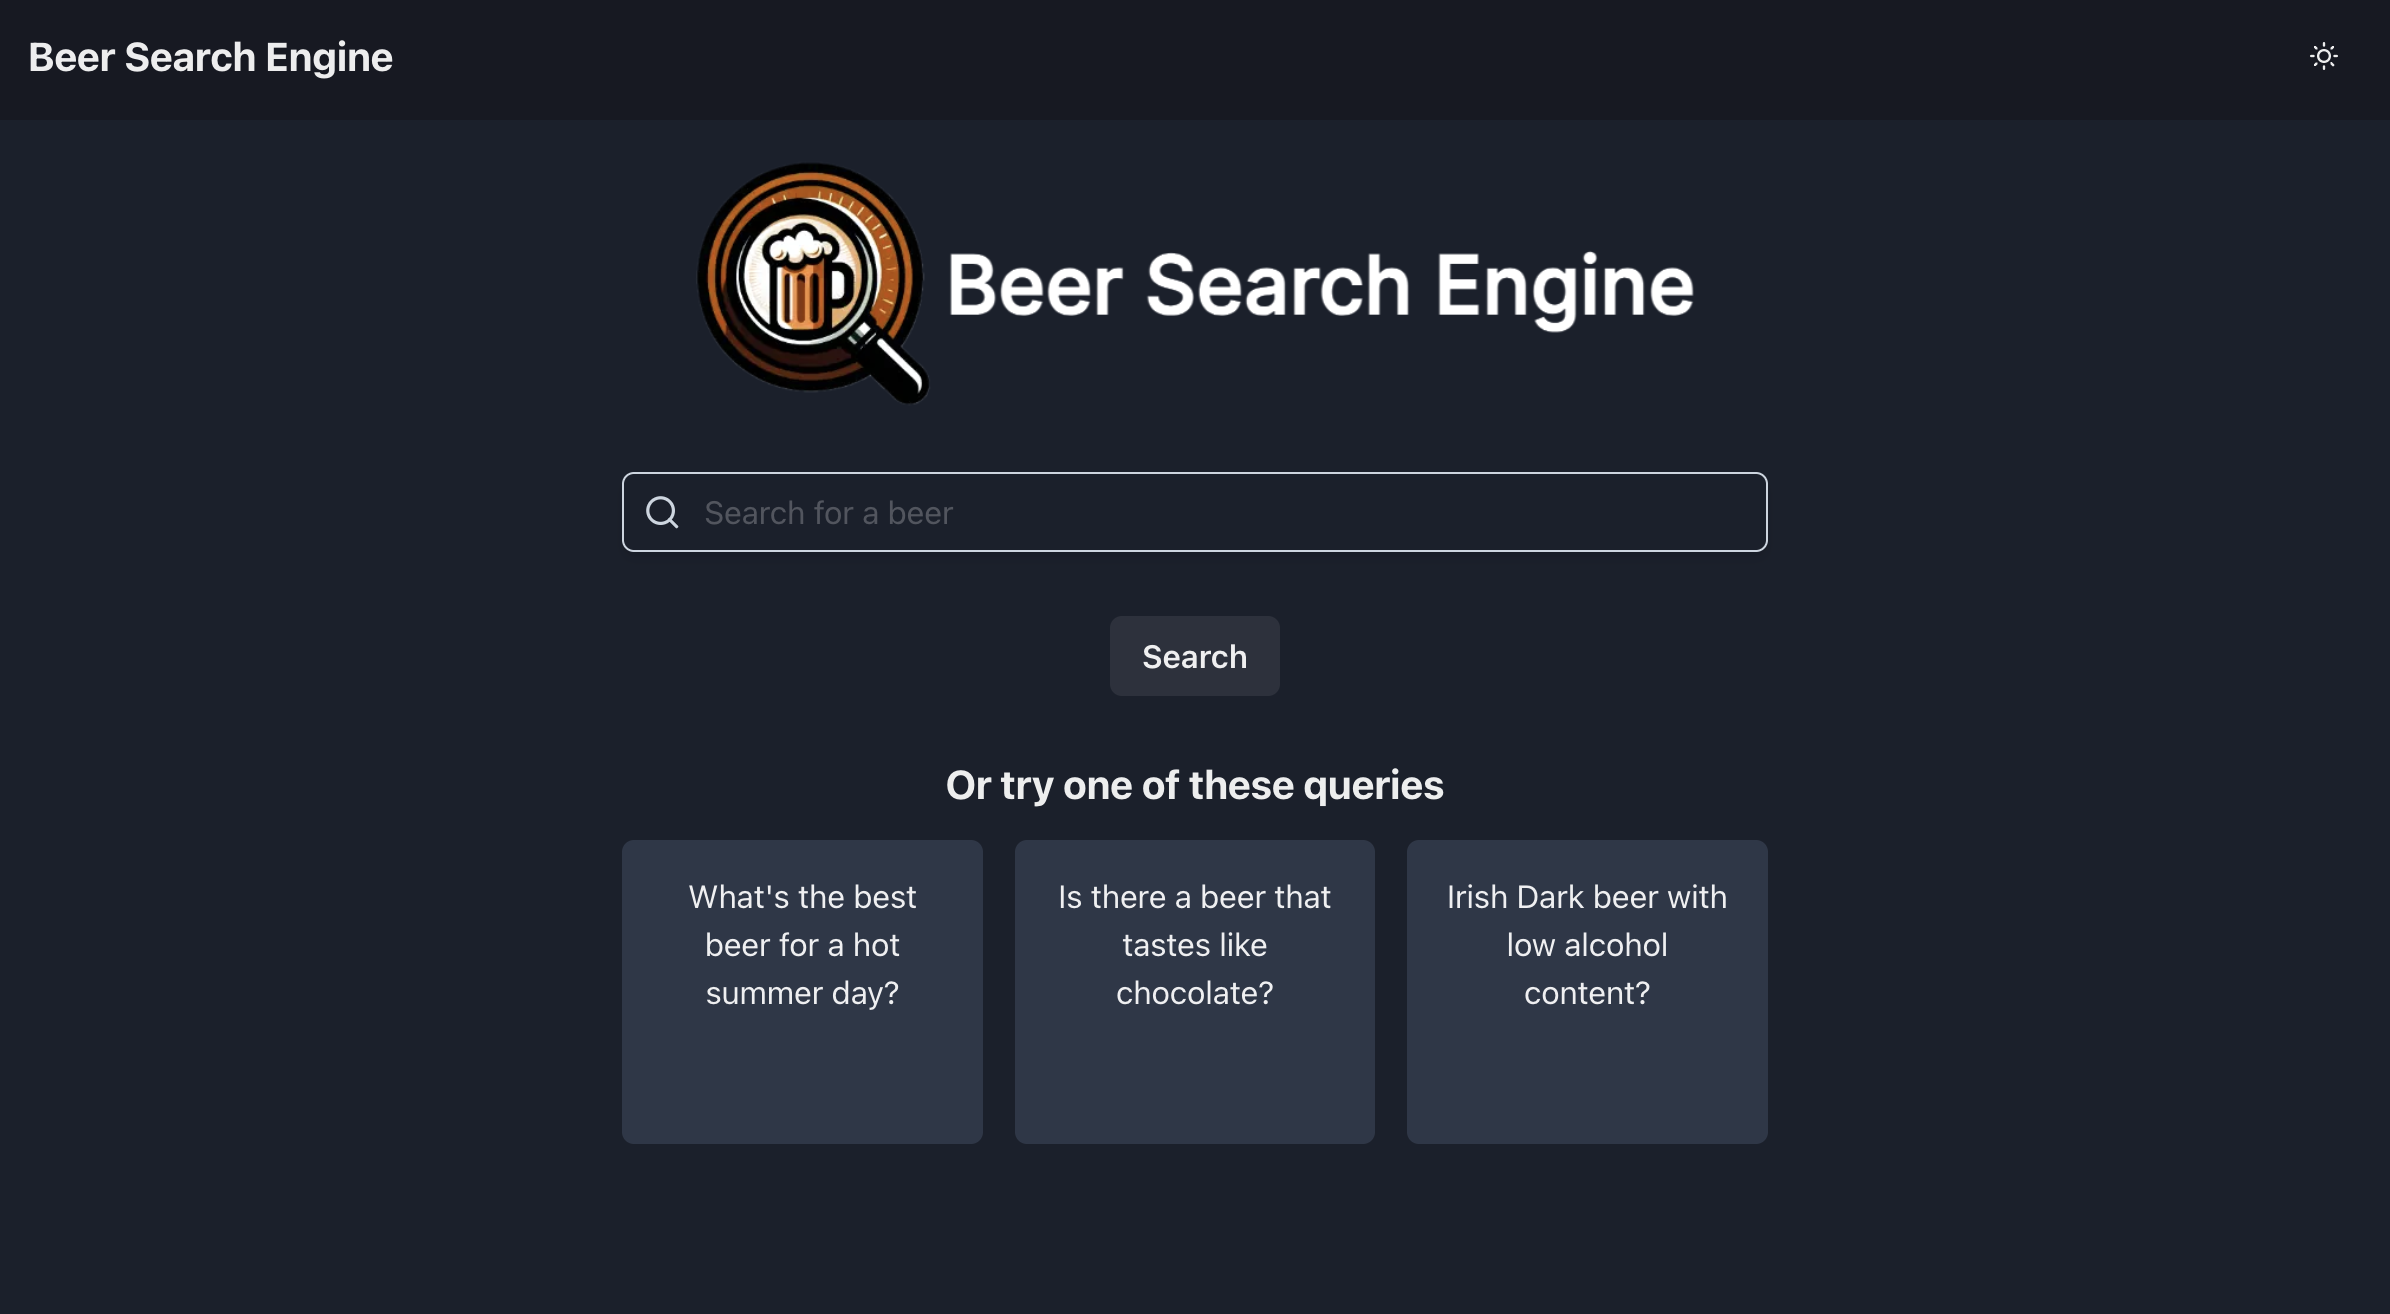
\includegraphics[width=1\textwidth]{img/3_implementation/homepage.png}
  \caption{Web interface homepage that allows the user to perform an initial search.}
  \label{fig:home-page}
\end{figure}

% Search page screenshot
\begin{figure}[H]
  \centering
  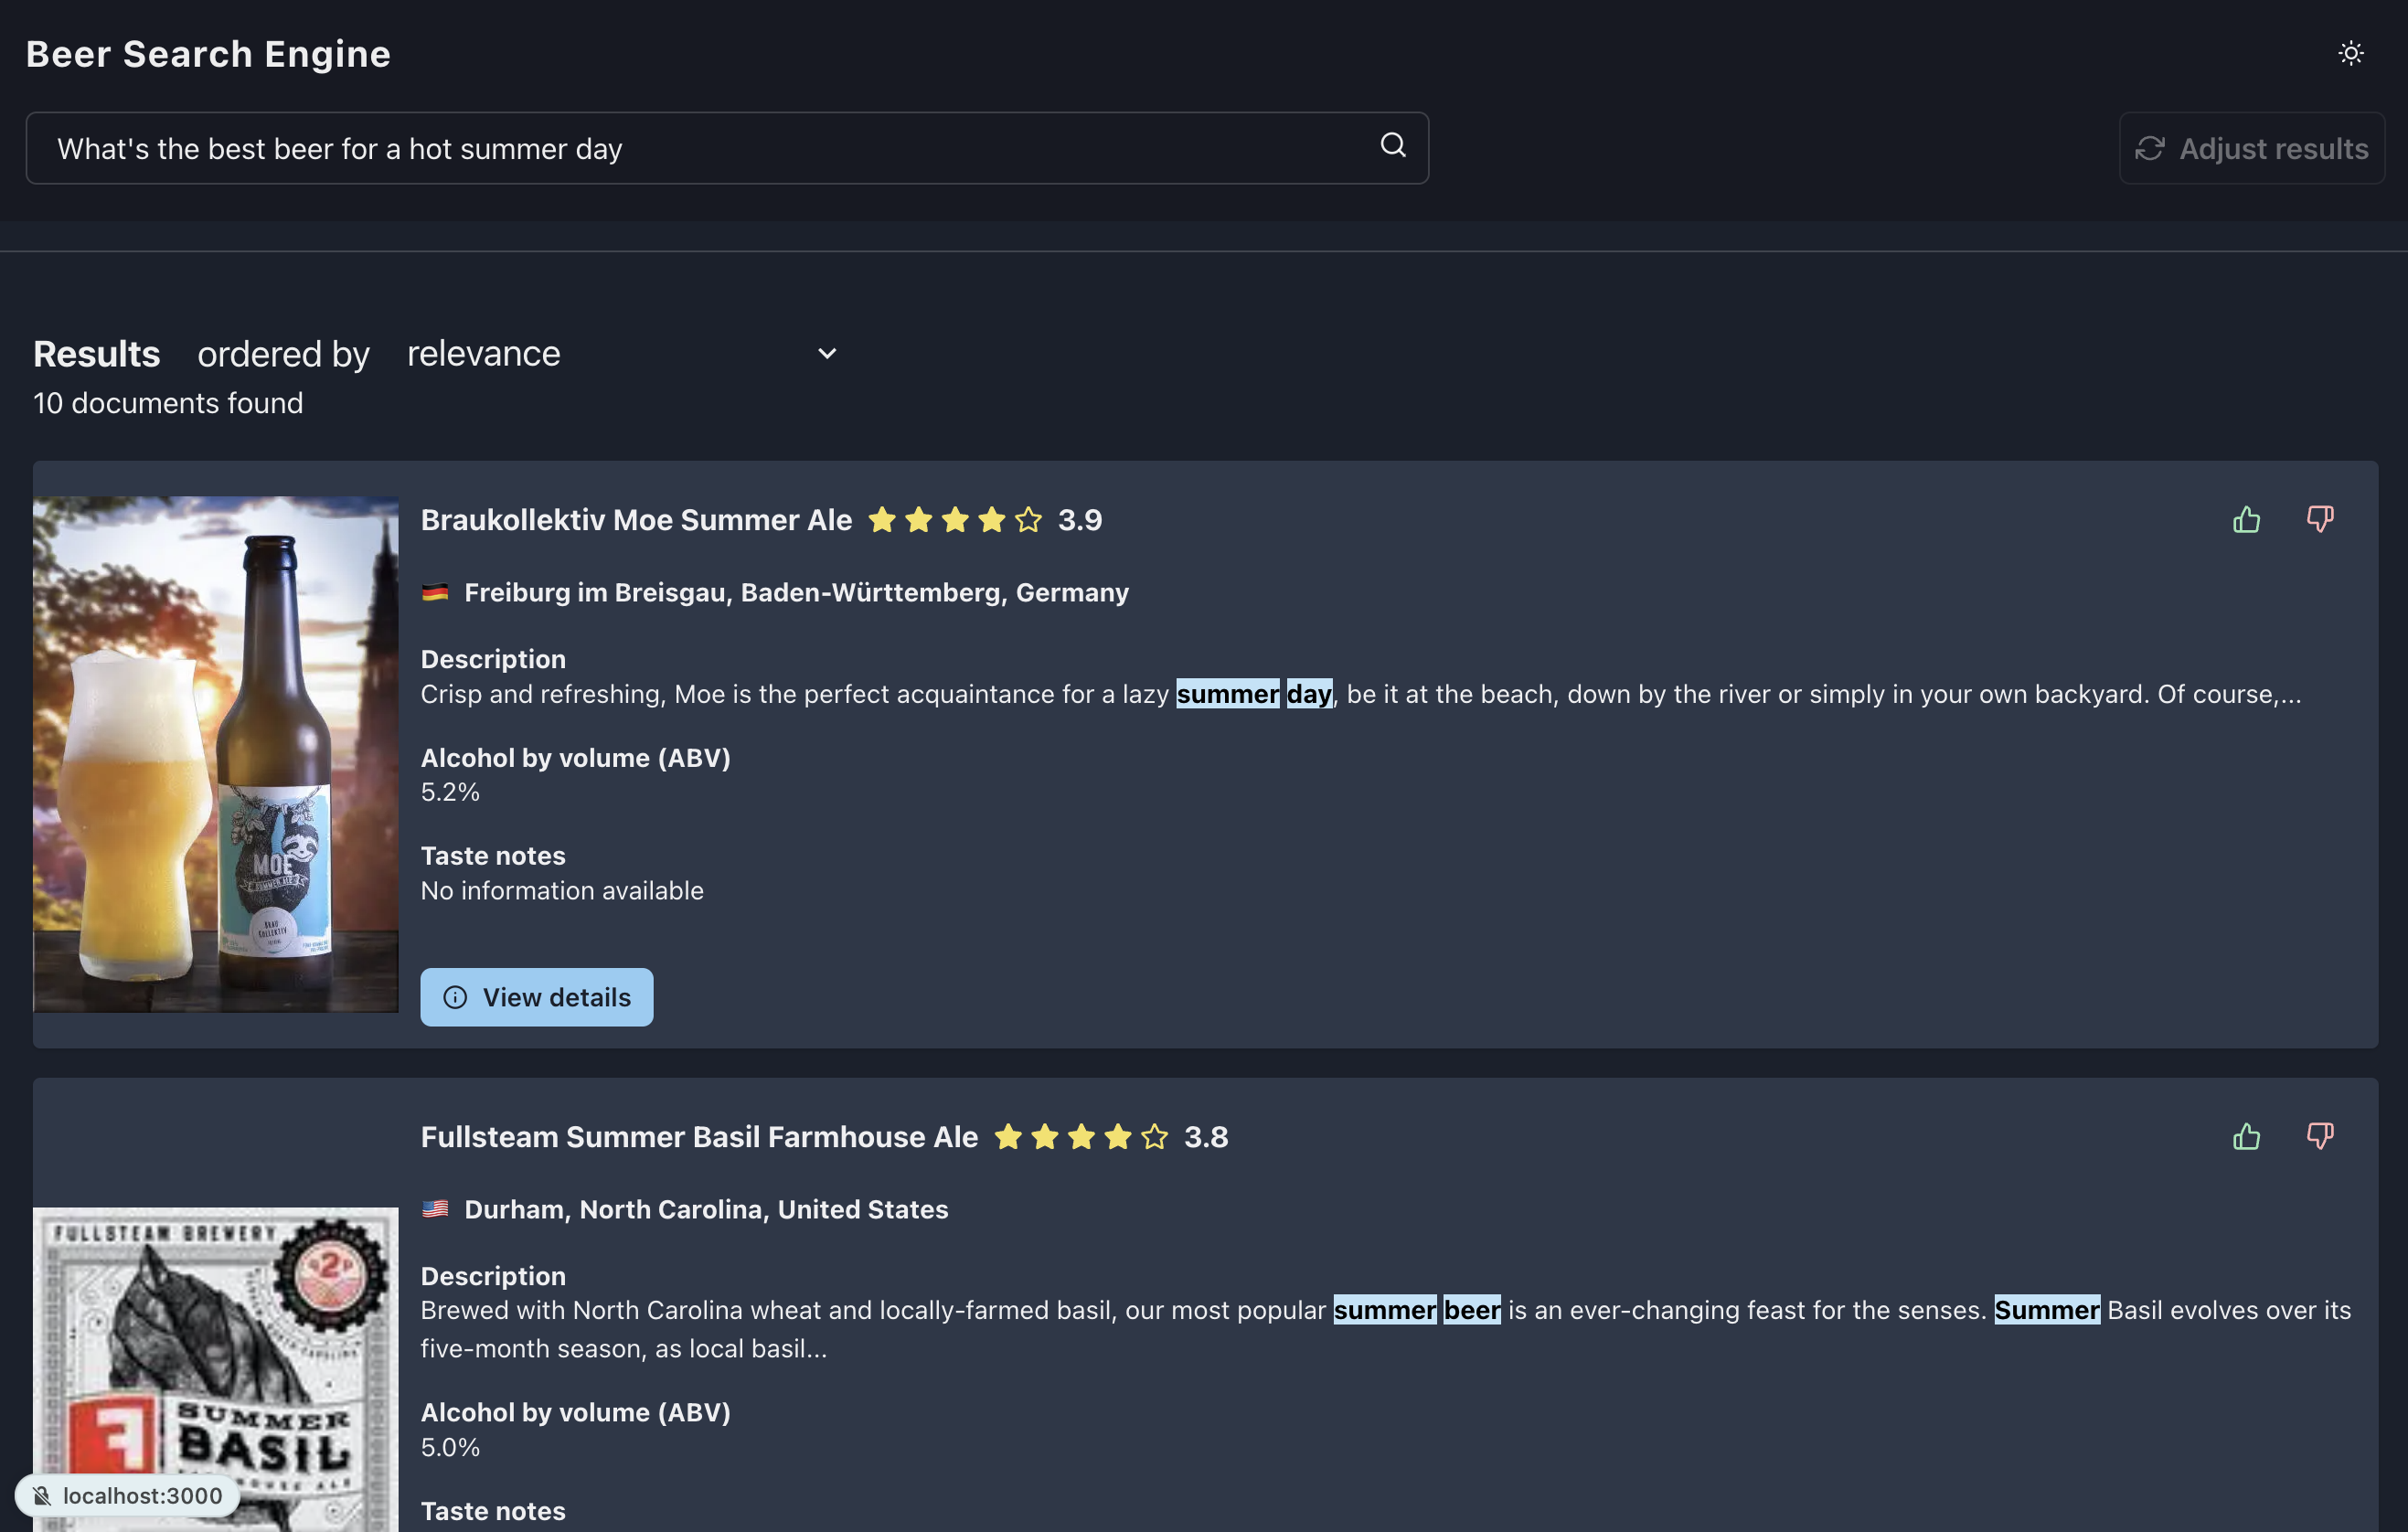
\includegraphics[width=1\textwidth]{img/3_implementation/search-page.png}
  \caption{Search page that allows the user to visualize the query results and perform relevance feedback on them to improve the results.}
  \label{fig:seach-page}
\end{figure}

\subsubsection{Features}

The search engine user interface offers the following features:

\begin{itemize}
  \item Simple and intuitive user interface that allows the user to perform a search in a matter of seconds.
  \item The user can perform relevance feedback to improve the results by explicitly specifying which results are relevant and which are not.
  \item The user can filter the results by multiple criteria: relevance (default), ABV (Alcohol By Volume), rating and name, allowing also to sort the results by ascending or descending order.
  \item Result snippets are provided to give the user a better understanding of why a result is relevant to the query by highlighting the present query terms.
  \item The entire interface supports both light and dark mode to provide a better user experience.
  \item Has been put a strong focus on accessibility, supporting screen readers and choosing colors that are accessible to visually impaired users (refer to Section \ref{sec:lighthouse-benchmark} for more details).
\end{itemize}

\subsubsection{Lighthouse benchmark}
\label{sec:lighthouse-benchmark}

To assess the quality of the frontend, a Lighthouse benchmark has been performed. Lighthouse is an open-source tool that allows to measure the performance, accessibility, best practices and SEO of a web application. The benchmark, focusing on the search page, has been performed on a \textit{MacBook Pro 16" 2023} with the following specifications:

\begin{itemize}
  \item \textbf{CPU}: Apple M2 Pro
  \item \textbf{RAM}: 16 GB
  \item \textbf{OS}: macOS Sonoma 14.0
\end{itemize}

In the following figure (Figure \ref{fig:lighthouse-benchmark}) is possible to see a partial screenshot of the benchmark results.

% Lighthouse benchmark
\begin{figure}[H]
  \centering
  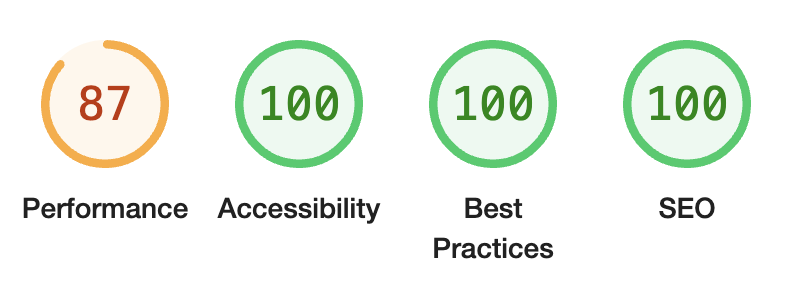
\includegraphics[width=.5\textwidth]{img/3_implementation/lighthouse-benchmark.png}
  \caption{Lighthouse benchmark of the search page of the frontend.}
  \label{fig:lighthouse-benchmark}
\end{figure}

From the results, it is possible to see that the frontend has a perfect score in three of the four categories: accessibility, best practices and \textit{SEO} (Search-Engine Optimization). Performance is the only area not scoring perfectly, mainly due to slow-loading image CDNs.

Slow-loading images are a common problem in web applications, and special measures have been taken to mitigate this issue: images are loaded asynchronously, and a placeholder is shown while the image is loading, allowing the user to browse the results without waiting for the images to load.

\newpage
\subsection{Flow of execution}

To allow readers to better understand the flow of execution of the system, Figure \ref{fig:flow-diagram} outlines how the system handles a user query and how it performs relevance feedback.

% Flow diagram of the system
\begin{figure}[H]
  \centering
  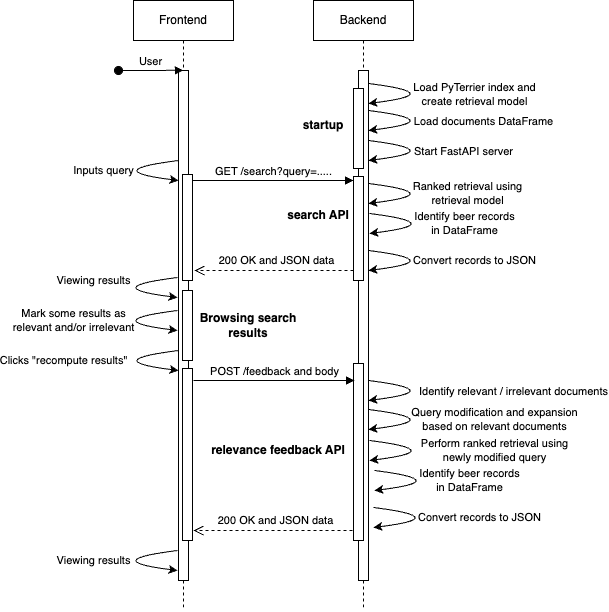
\includegraphics[width=1\textwidth]{img/3_implementation/search-flow.png}
  \caption{Flow diagram describing the execution of the system when a user performs a search and relevance feedback.}
  \label{fig:flow-diagram}
\end{figure}
\newpage

\section{Evaluation}

\subsection{Evaluation metrics}

\subsection{System Usability Scale (SUS)}

\subsection{User Experience (UX) questionnaire}



\end{document}
